\newpage
\chapter{Video Face Clustering for Subtitles Positioning in 360-Videos}
\label{chap:subtitles_positioning}

In \cite{mendes2020authoring}, we proposed an authoring model for interactive 360-video. In such a model, we can define interactive 360-videos that are presented together with additional information attached to it, such as images, text, subtitles, 2D traditional videos, and spatial audio. The positioning of such information is defined by their polar coordinates, start time, and duration. For instance, we can define that a text moves with the user's head motion and is always visible or that such text is placed at a fixed position if it is in the user's field of view. In this chapter, we describe how \emph{video face clustering} can be used together with this authoring model for automatic subtitles positioning in 360-video. Section \ref{sec:authoring_clustering_360} describes how we adapt \emph{Video Face Clustering} for the context of 360-videos. In Section \ref{sec:authoring_model}, we describe the authoring model we proposed that together with \emph{Video Face Clustering} can be used for automatic positioning subtitles in 360-videos.
 
\section{Video Face Clustering in 360-Videos}

\label{sec:authoring_clustering_360}

Nowadays, the most common way for representing and transmitting 360-video is using equirectangular projection~\cite{yang2018object}. With the equirectangular projection, each sphere point is defined by two angles~\cite{snyder1987map}: \emph{latitude}~$\theta \in [-90^{\circ}, +90^{\circ}]$ and \emph{longitude}~$\phi \in [-180^{\circ}, +180^{\circ}]$. This kind of projection creates challenges for image processing and computer vision algorithms, especially to the convolution-based ones because of the severe distortions in areas vertically distant from the center of the image~(see Figure \ref{fig:equirectangular_proj}). Due to these distortions, we adapted the \emph{Face Detection} step of our method which uses a traditional CNN. Section \ref{subsec:360_face_detection} describes how we adapted the \emph{Face Detection} step to the 360-video context.

\begin{figure}[!ht]
\centering
    \begin{subfigure}{0.47\linewidth}
        \centering
        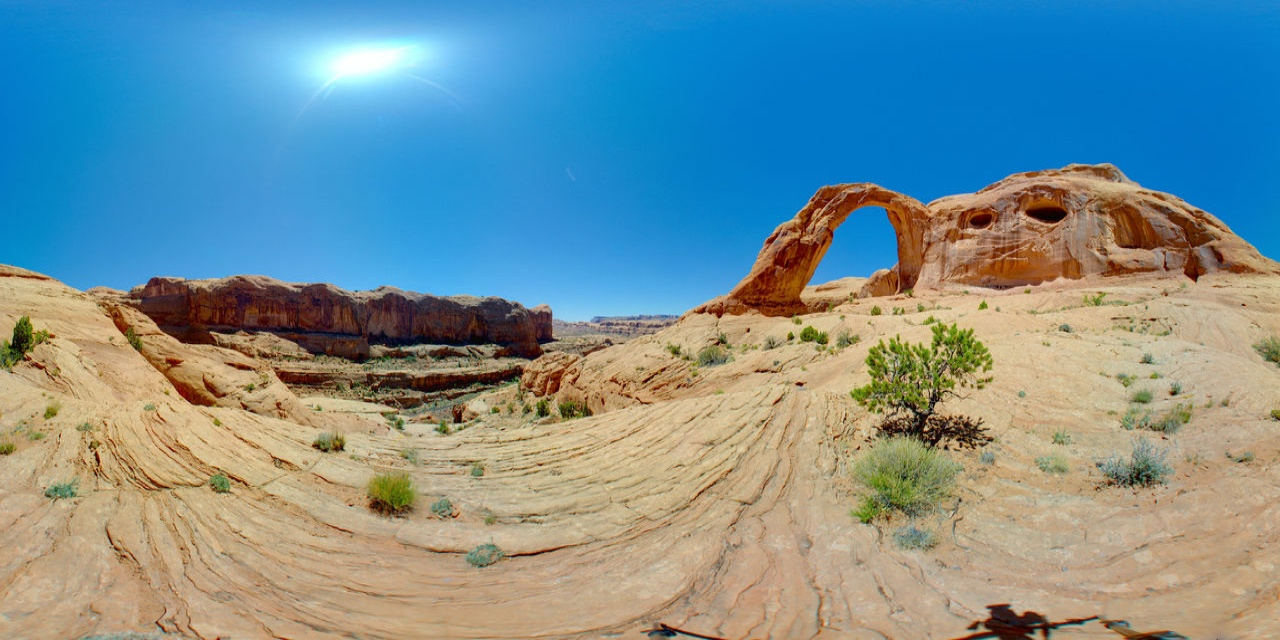
\includegraphics[width=1\textwidth]{img/video360/equi_outdoor.jpg}
        \caption{Outdoor equirectangular image.}
        \label{subfig:out_equi}
    \end{subfigure}\hfill
    \begin{subfigure}{0.47\linewidth}
        \centering
        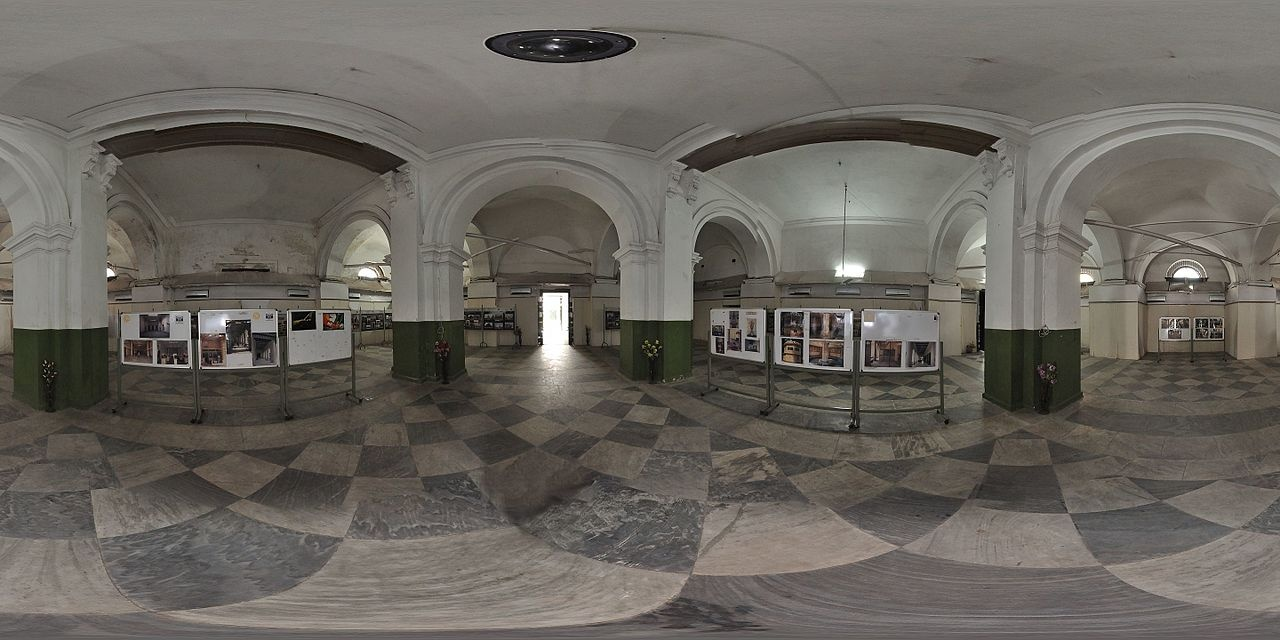
\includegraphics[width=1\textwidth]{img/video360/equi_indoor.jpg}
        \caption{Indoor equirectangular image.}
        \label{subfig:in_equi}
    \end{subfigure}

\caption{Examples of 360-images represented through equirectangular projection.}
\label{fig:equirectangular_proj}
\end{figure}

\subsection{Face Detection in Equirectangular 360°}
\label{subsec:360_face_detection}

In order to mitigate the problem of severe distortions present in the equirectangular projection, we have used an approach based on viewports extraction. Figure \ref{fig:360_face_detection} shows this process and each of its steps is explained in the following paragraphs.

\begin{figure}[!ht]
    \centering
    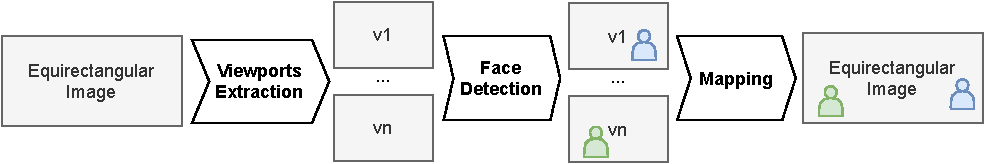
\includegraphics[width=1\linewidth]{img/video360/360facedetection.pdf}
    \caption{360-degree face detection process.}
    \label{fig:360_face_detection}
\end{figure}

Given an equirectangular image, which could also be a frame from a 360-video, we first perform \emph{Viewports Extraction}. A viewport represents a portion of the 360-degree scene~(see Figure \ref{fig:authoring_exviewport}), it is similar to when a person takes a picture in the real world. The picture represents the world from a point of view towards a specific direction. A viewport is defined by its center, in polar coordinates (lat, long), its field of view~(FoV), and the width or height of the resulting image.

\begin{figure}[!ht]
    \centering
    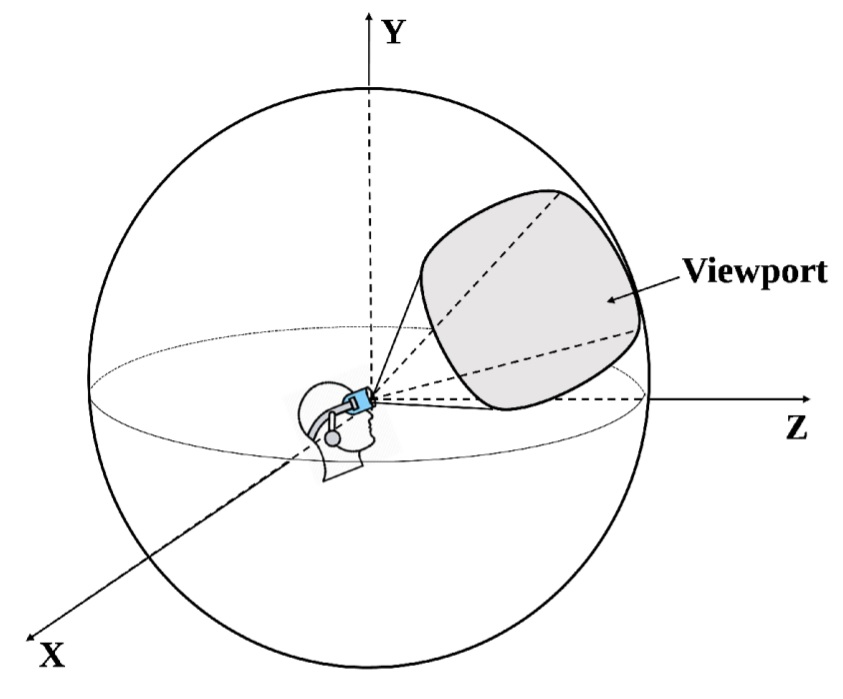
\includegraphics[width=0.5\linewidth]{img/video360/viewport.jpg}
    \caption{Example of a viewport from a 360-video. Extracted from Nguyen \emph{et al.} \cite{nguyen2020evaluation}.}
    \label{fig:authoring_exviewport}
\end{figure}

Because we want the viewports to cover the greatest possible area from the 360-degree image, our method receives two parameters: the viewports' \emph{density}~(\emph{d}) and \emph{FoV}. The \emph{density} is equal to the number of viewports in the latitude range. Proportionally, the number of viewports in the longitude range is equal to double the \emph{density}. Figure \ref{fig:authoring_viewports} shows viewports extracted from Figure \ref{subfig:out_equi} with \emph{density}=3 and FoV=60°. As the density was equal to three, the number of viewports is three in the latitude range and six in the longitude range. In total, 18 viewports were extracted in the example below.

\begin{figure}[!ht]
    \centering
    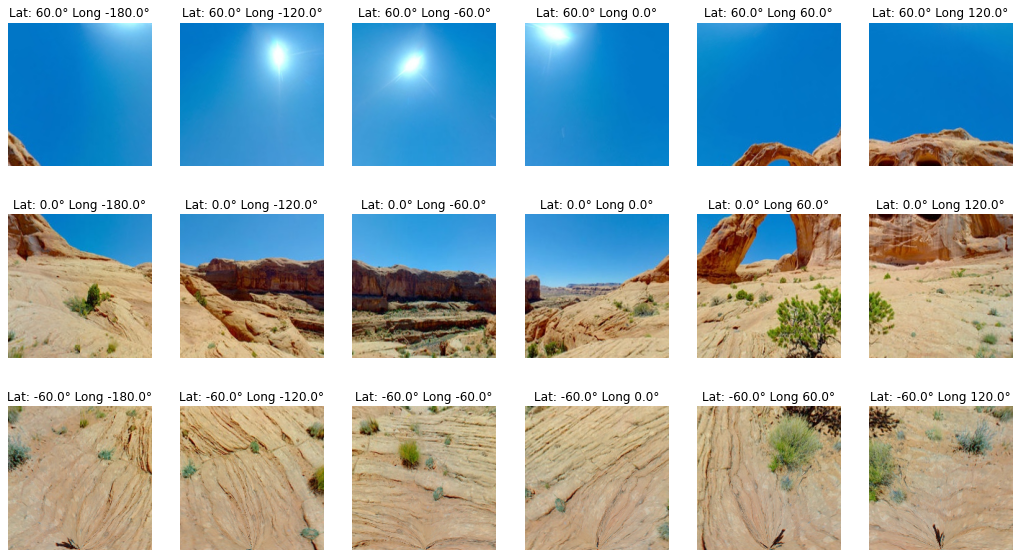
\includegraphics[width=1\linewidth]{img/video360/viewports.png}
    \caption{Viewports extracted from Figure \ref{subfig:out_equi} with \emph{density}=3 and FoV=60°.}
    \label{fig:authoring_viewports}
\end{figure}

With these viewports, we aim at reducing the distortions since we are representing the equirectangular image with a series of standard images, similar to the ones used by traditional CNNs. Next, for each of these viewports, we perform \emph{Face Detection} using a traditional CNN. Then, for each viewport we have a group of faces detected.

In the last step of our approach, called \emph{Mapping}, we map each face detected back to the equirectangular image. One can notice that some parts of the equirectangular image are present in more than one viewport. Notice that the sun is present in three viewports in the first line of Figure \ref{fig:authoring_viewports}. To avoid repeated detections in the equirectangular image, we use the Non-Maximum Supression~(NMS) algorithm. This algorithm eliminates overlapping bounding boxes within a given threshold and is widely used in object detection algorithms~\cite{nms1, nms2, nms3, nms4, nms5}.

We evaluated this approach in comparison to applying a detection model directly to the equirectangular image. We searched for datasets for face detection in equirectangular 360-images. However, by the time of our search, we have not found any. For that reason, we decided to create a synthetic dataset to perform this evaluation. 
%%
Similar to Fu \emph{et al.} \cite{fu2019fddb}, we created a synthetic dataset based on the Face Detection Data set and Benchmark~(FDDB)~\cite{jain2010fddb}. Fu \emph{et al.} \cite{fu2019fddb} create a synthetic dataset for face detection in 360-degree fisheye images. Ours, differently, aims at equirectangular images, projecting standard images to the equirectangular projection.

The FDDB dataset~\cite{jain2010fddb} is a popular benchmark for face detection evaluation containing 2845 images and 5171 faces. We collected 19 indoor and outdoor equirectangular images from Google Images,\footnote{\url{https://www.google.com/imghp}} ESO,\footnote{\url{https://www.eso.org/public}} and PxHere\footnote{\url{https://pxhere.com}} to use as background.
%%
For each image in the FDDB dataset, we randomly chose a latitude, longitude, and equirectangular background image to project it following the projection to equirectangular described in the work of Su \emph{et al.} \cite{su2017learning}.
%%
For each face present on the FDDB image, we projected its bounding box to the new equirectangular synthetic image. Figure \ref{fig:authoring_fddb_proj} shows an example of an image from FDDB projected in the polar coordinates \emph{lat} $ = -60^{\circ}$ \emph{long} $ = 0^{\circ}$ to an equirectangular image.

\begin{figure}[!ht]
\centering
    \begin{subfigure}{0.4\linewidth}
        \centering
        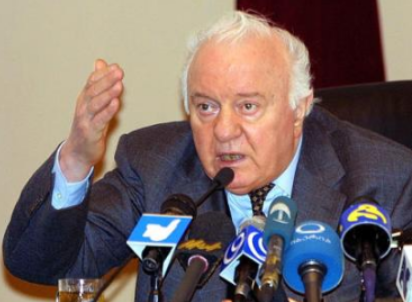
\includegraphics[height=9em]{img/video360/face_pre.png}
        \caption{FDDB image example.}
        \label{subfig:face_pre}
    \end{subfigure}\hfill
    \begin{subfigure}{0.55\linewidth}
        \centering
         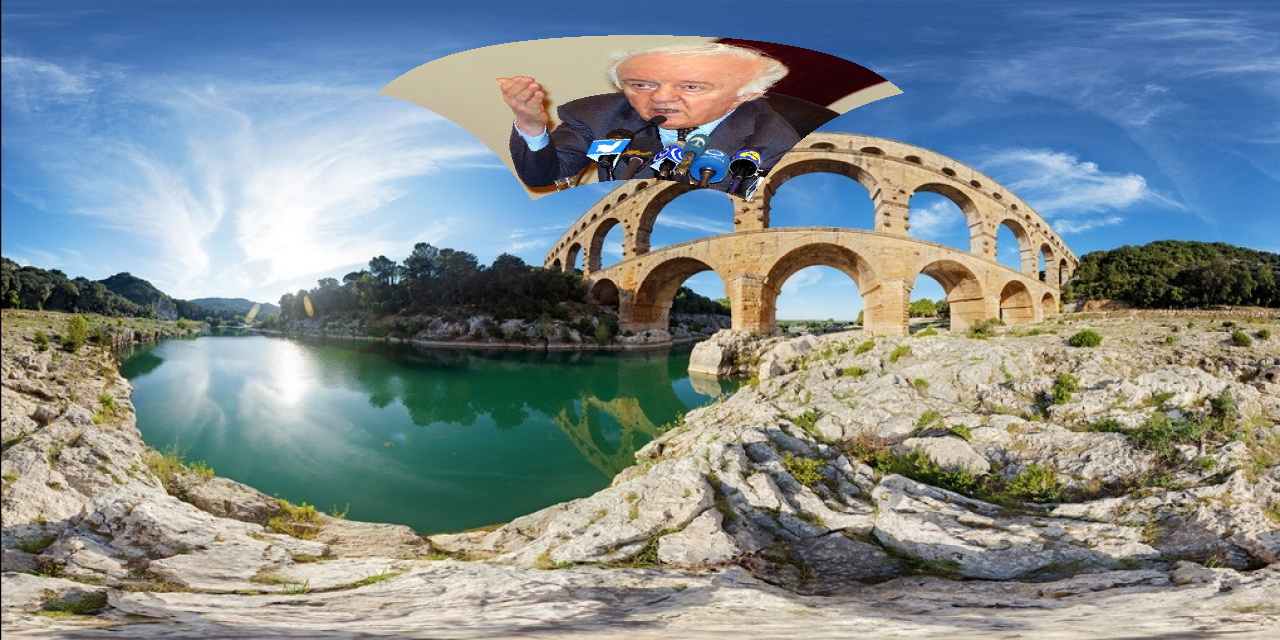
\includegraphics[height=9em]{img/video360/face_pos.png}
        \caption{Projection example of FDDB image.}
        \label{subfig:face_pos}
    \end{subfigure}

\caption{FDDB image projection to Equirectangular image.}
\label{fig:authoring_fddb_proj}
\end{figure}

Depending on the position that the traditional FDDB image is projected, the distortions are more or less severe. The distortions increase as the projection vertically distances from the center of the equirectangular image. Figure \ref{fig:different_projections} shows different resulting equirectangular images depending on the projection position. Notice that the projections vertically close to the border of the image have more distortions than the ones close to the center of the image.

\begin{figure}[!ht]
    \centering
    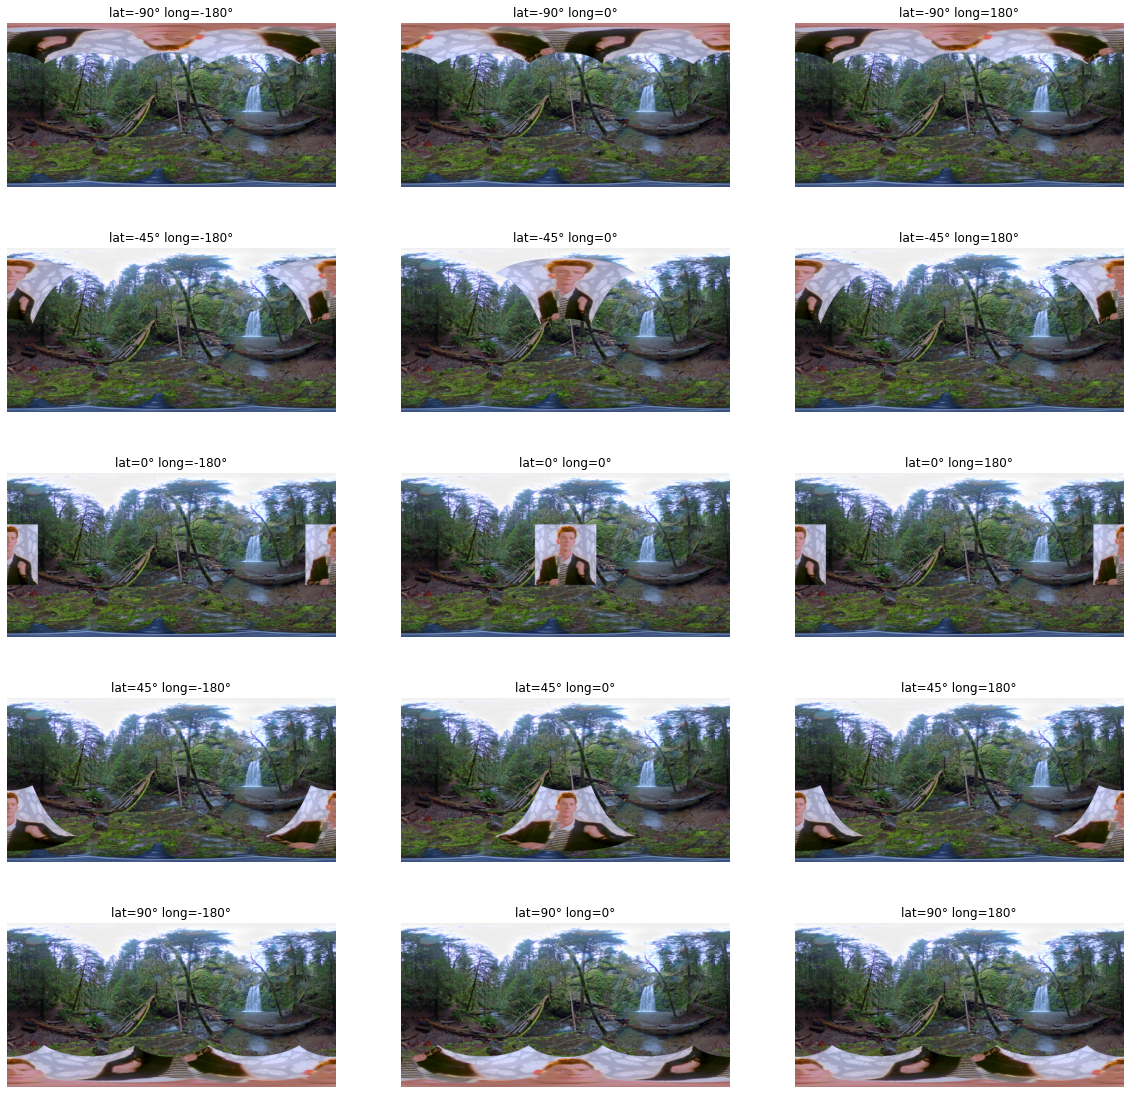
\includegraphics[width=1\linewidth]{img/video360/different_projections.png}
    \caption{Different resulting synthetic equirectangular images depending on the position that the rectlinear image was projected.}
    \label{fig:different_projections}
\end{figure}

We evaluated our approach in the synthetic dataset using MTCNN\cite{mtcnn} as the model for face detection. We compare the usage of MTCNN alone, directly in the equirectangular images, against MTCNN with viewports. For the MTCNN with viewports, we used extracted viewports with \emph{density}=3 and FoV=60°. We evaluated both methods using the Mean Average Precision~(mAP) that is widely used for the object detection task~\cite{map1, map2, map3, map4}. 


From Figure \ref{fig:different_projections}, one can notice that a greater module of the latitude~($|lat|$) implies more severe distortions, as the projection is more vertically distant from the center of the equirectangular image. Figure \ref{fig:results_360_detection} shows the results we obtained for MTCNN and MTCNN with viewports. 
We vary the x-axis of the chart so that we consider only the synthetic equirectangular images whose projection's $|lat|$ is greater than or equal to each x. In this way, a greater x means a more difficult subset of images from our synthetic dataset. The mAP value for MTCNN drops drastically as we start considering only more and more difficult images. In contrast, with the use of viewports, the mAP value still decreases but at a slower pace. Besides achieving better results, one of the main advantages of this technique is that it can be used with a model that was trained for detecting faces in traditional images.

\begin{figure}[!ht]
    \centering
    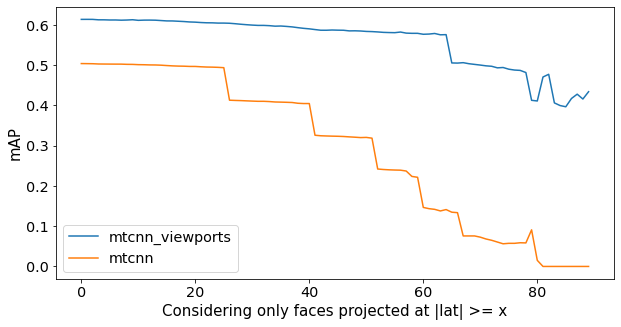
\includegraphics[width=0.8\linewidth]{img/video360/results_360_detection.png}
    \caption{Face detection results using MTCNN and MTCNN with viewports.}
    \label{fig:results_360_detection}
\end{figure}

With this adaptation, we can use \emph{Video Face Clustering} for 360-video. To do that, in the \emph{face detection} step we use the viewports strategy with MTCNN. 


\section{An Authoring Model for Interactive 360-Videos}
\label{sec:authoring_model}

In this section, we describe an authoring model for interactive 360-videos. Although the model is not entirely used for subtitles positioning in 360-videos, we describe it completely because the development of such an authoring model was part of the researches conducted during our master research.

Despite the limited ``look around'' interactivity supported by traditional 360-videos and HMDs, \emph{interactive 360-videos}~\cite{chambel2011,berning2013parnorama} support additional interactive elements, such as overlaid 2D/3D information, hyperlinks, and additional input elements.
%%
Such features allow an enhanced user experience, supporting applications such as remote operations and telepresence, museums, immersive interactive narratives, and improve educational content.
%%
Most of the current 360-video streaming services, however, still do not support such interactive features for 360-videos.
%%
Indeed, when compared to its 2D-only video counterpart, although most of the popular streaming services~(e.g., Youtube and Facebook) offer tools to create interactive 2D videos (\emph{e.g.}, to insert additional information, subtitles, and hyperlinks), they lack similar tools to create interactive 360-videos.

We propose a declarative authoring model that allows authors to design and create interactive 360-videos.
%%
First, we analyze different scenarios of immersive multimedia applications based on 360-videos intending to extract the main requirements for such an authoring model.
%%
Then, based on the gathered requirements, we propose an XML-based declarative model that allows authors to design and create 360 interactive videos.

\subsection{Scenarios and requirements}
\label{subsec:authoring_scenarios}

The following target scenarios are used to gather the requirements for our authoring model for interactive 360-videos.

\textbf{360 hypervideo}.
%%
This scenario is characterized by navigation among 360-videos, and can be useful, for instance, in entertainment or educational context~(see Figure \ref{fig:cenario_hiper}). The user can navigate from the current to another 360-video, while the current one proceeds in a ``preview mode''. Besides the support for navigation between 360-degree videos, it should be possible to add overlaid information to it~(e.g., image, video, text) to enhance its viewing experience. An example of such a scenario is a virtual tour in a museum, where the user may navigate through different rooms. Each room could have additional information about the presented piece of art. Another example is a virtual learning environment, in which the user can navigate among different topics and learn more about each of them with additional information.

\begin{figure}[!ht]
    \centering
    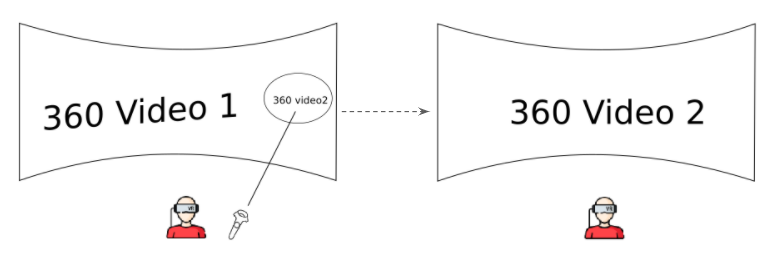
\includegraphics[width=0.65\linewidth]{img/video360/hyper.png}
    \caption{360 hypervideo scenario.}
    \label{fig:cenario_hiper}
\end{figure}

\textbf{Accessible 360-video}. 
%% 
In this scenario, a 360-video is presented together with its translation in either sign language or subtitles~(see Figure \ref{fig:cenario_acessivel}). For the sign language case, both a 2D regular video using Picture-in-Picture~(PiP) or a 3D human model could be displayed. Such a scenario intends to provide an immersive experience for people with hearing disabilities. An example is a voice-based virtual tutorial for managing a machine in a factory that can support sign languages or subtitles to allow the inclusion of people with hearing disabilities.

\begin{figure}[!ht]
    \centering
    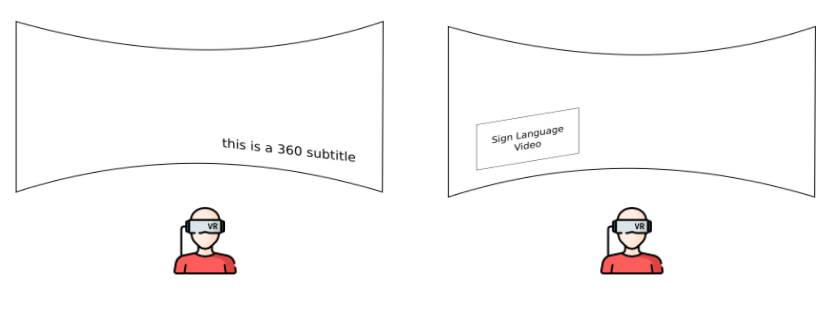
\includegraphics[width=0.65\linewidth]{img/video360/accessible.png}
    \caption{Acessible 360-video scenario.}
    \label{fig:cenario_acessivel}
\end{figure}

\textbf{360-video with guided attention}.
In this scenario, a 360-video has a recommended region to look at. Whenever the user is not looking at the recommended region, additional guiders (e.g., arrows) can be rendered informing the user to where he should be looking in the 360-video~(see Figure \ref{fig:cenario_guiado}). Also, a live view of it can be presented in picture-in-picture~(PiP) in part of the field of view; thus, providing the user with key content, whether he/she is looking at it or not. Besides visual cues, spatial audio cues are also important in virtual environments and can help guide users' attention. Thus, the audio of the 360-degree video may come from the recommended position, in a way that it sounds different depending on the position the user is looking at. To support such a scenario, it should be possible to detect if the user is looking in a specific direction of the scene and to render another segment of the video using PiP. The region of interest of a 360-degree video is content-dependent, thus the producer should be able to customize it towards providing the best possible user experience. An example of such a scenario is a lecture, in which the recommended position to look at is where the lecturer may be located, e.g. the stage.

\begin{figure}[!ht]
    \centering
    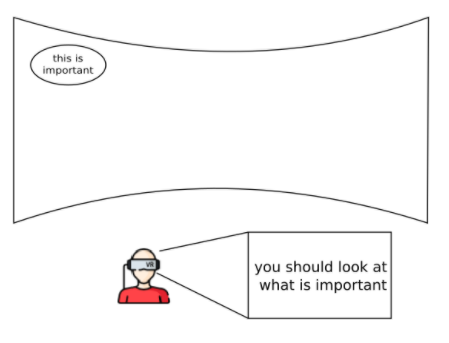
\includegraphics[width=0.5\linewidth]{img/video360/guided.png}
    \caption{360-video with guided attention scenario.}
    \label{fig:cenario_guiado}
\end{figure}

Based on the above target scenarios, we can extract requirements addressing presentation~(RP) and interaction~(RI) that should be supported by an authoring model for 360 interactive videos, which are detailed in what follows.

\begin{itemize}
    \item \textbf{RP.1 Overlaid information}. Additional media objects (video, image, sound, and text) might be positioned in the 360-degree environment.
   \item \textbf{RP.2 Styling}. Different media elements may share the same position and presentation characteristics. Thus, the author should be able to reuse the same style in different elements.
  \item \textbf{RP.3 3D Audio}. A 3D audio manipulates the sound delivered by stereo speakers or headphones, creating the idea that the audio is coming from a specific direction.
  \item \textbf{RP.4 Subtitles}. Support subtitles positioning in 360-video.
  \item \textbf{RP.5 360 Spatial Layout}. The media elements should use a 360-based coordinate system, whereas the viewer camera is the center.
  \item \textbf{RP.6 Presentation Timing}. The media elements should be presented synchronized with the 360-video of the scene. 
  \item \textbf{RI.1 Navigation}. This requirement intent to enable users to navigate between 360-videos. This also includes showing them a preview of possibles videos to visit.
  \item \textbf{RI.2 Hotspot}. This requirement defines a position in the 360-degree scene in which different actions can be performed when the user looks at it or is not looking at it.
  \item \textbf{RI.3 Viewport preview}. This requirement refers to the use of a picture-in-picture live view at the user's current viewport, rendering an important section of the 360-degree scene defined by a \emph{hotspot}.
\end{itemize}



\subsection{Proposed model}
\label{subsec:proposal}
 
To fulfill the aforementioned requirements, we propose an authoring model that allows authors to design and create 360 interactive videos. Table~\ref{tbl:entities} presents the entities of the model.
\begin{table}[!ht]
\footnotesize
\begin{tabularx}{\linewidth}{ p{3cm} p{4cm} X }
\hline

\textbf{element} & \textbf{children} & \textbf{attributes}\\ \hline

\textbf{\emph{presentation360}}  & \emph{head}, \emph{\emph{body}} &  \\ \hline

\textbf{\emph{head}}  & \emph{style} &  \\  \hline

\textbf{\emph{style}}  &  & * \\  \hline

\textbf{\emph{body}}  & \emph{scene360}+ & entry \\ \hline

\textbf{\emph{scene360}}  & \emph{text}*, \emph{image}*, \emph{video}*,
\emph{subtitle}*, \emph{preview}*, \emph{hotspot}*, \emph{mirror}* & src, volume? \\  \hline

\textbf{\emph{text}, \emph{image}}  &  & 
id, src, r?, phi?, theta?, tpos?, style?, begin?, dur?, followCamera?, onselect? \\ \hline

\textbf{\emph{audio}, \emph{video}, \emph{subtitle}, \emph{preview}}  &  & 
id, src, r?, phi?, theta?, tpos?, style?, begin?, dur?, followCamera?, onselect?, clipBegin?, clipEnd?\\ \hline

\textbf{\emph{mirror}}  &  & 
id, src, r?, phi?, theta?, tpos?, style?, begin?, dur?, 
followCamera? \\ \hline

\textbf{\emph{hotspot}}  &  & 
id, src, r?, phi?, theta?, tpos?, 
style?, begin?, dur?,  onLookAt?, duringNotLookingAt?, onSelect? \\ \hline

\hline
 \end{tabularx}
\caption{Elements BNF. Conventionally: a \emph{plus sign} (+) indicates that the element can occur one or more times. The \emph{asterisk} (*) indicates that the element occurs zero or more times. Optional attributes (may not exist or have an occurrence) appear with a \emph{question mark} (?) unlike the others that are mandatory. 
}
\label{tbl:entities}
\end{table}

\emph{<presentation360>} is the root element of our model. It has two children elements: \emph{<head>} and \emph{<body>}. Similar to other declarative multimedia languages~(\emph{e.g}., HTML, SMIL~\cite{ayers2001synchronized}, and NCL~\cite{soares2006nested}), the reusable elements inside the \emph{<head>} and the structured content inside the \emph{<body>}.

In the \emph{<head>},  reusable objects can be grouped by the <style> element, which can be seen as a macro in which any of the media attributes may be defined (\textbf{RP.2}). Then, any element may reuse these attributes assigning their \emph{style} attribute to the \emph{id} of a previously defined \emph{<style>}.

The <\emph{body}> element is composed of different \emph{\emph{<scene360>}} elements. Its \emph{entry} attribute indicates the identifier of \textit{<scene360>} that starts with the application. The \emph{<scene360>} element is defined by its \emph{id}, \emph{src}~(source of the 360-degree video) and \emph{volume} (varying from 0 to 1). Each scene is composed of a set of media objects and the temporal behavior of those objects~(\textbf{RP.1}). In its current version, we support text, image, video, audio, and subtitle media objects, each one with its respective XML element~(see Table~\ref{tbl:entities}). The following attributes are shared by all media elements:

\begin{itemize}
  \item \emph{id}: the identifier by which the element is referenced by other elements.
  \item \emph{r, phi, theta}: define the element initial 360 spatial position.
  \item \emph{tpos}: it determines how the element moves through the 360-video's duration by pointing to a file that specifies 360 positions for predetermined moments in time. Such positions are relative to the initial \emph{r, phi, theta}.    
  \item \emph{begin}: the time, in seconds, in which the element is started relatively to the 360-video it is a child of.
  \item \emph{dur}: the duration, in seconds, of the element.
  \item \emph{clipBegin, clipEnd}: define that will be presented only a portion from sourced media.
  \item \emph{followCamera}: a Boolean attribute that, if \emph{true}, makes the element moves with the camera. Such movement creates the impression that the element is fixed for the user.
  \item \emph{onselect}: it refers to the \emph{id} of a 360-degree interactive video in a way that when the element is selected (using controllers of an HMD), the user is transported to the referred 360-degree interactive video.
\end{itemize}

Besides the above attributes, individual media objects can also have additional attributes. For instance, \emph{<image>}, \emph{<video>} and \emph{<audio>} have the attribute \emph{src}, that refers to the file source of the media object; \emph{<audio>} and \emph{<video>} have the attribute \emph{volume}, that defines the volume of such media objects, varying from 0 to 1. \textit{<audio>} also has a 3D behavior (\textbf{RP.3}), in a way that the user perceives the position in which it is placed. 3D Audio, also referred as spatial audio, is considered itself a type of immersive content~\cite{hughes_disruptive_2019}. \emph{<subtitle>}, \emph{<preview>} and \emph{<mirror>} are non-traditional objects. The \emph{<subtitle>} element has also a \emph{src} attribute that refers to an SRT~(SubRip Subtitle Format) file (\textbf{RP.4}). \emph{<preview>} and \emph{<mirror>} refer to other elements from the scene and have specific behaviors.

In our 360 spatial model (\textbf{RP.5}), the media objects are positioned using a polar coordinate system. Figure \ref{fig:polar_coordinates} shows the definition of the polar coordinates of a point $C$, which represents the center of a media object. $C1$ is the projection of $C$ on the $xz$ plane, while $C2$ is the projection on the $yz$ plane. Each \emph{r} attribute value specifies the radius of an imaginary sphere where the media objects are positioned. All of those spheres are concentric. The angles are defined based on the segment that goes from the origin to the edge. The attribute \emph{phi}~($\phi$) specifies the horizontal angle~(or longitude, in degrees) from that segment to the one that goes from $C1$ to the origin. Similarly, the attribute \emph{theta}~($\theta$) defines the vertical angle~(or latitude), but using $C2$.  The camera is positioned at the center of that coordinate system ($0$, $0$, $0$) and has a field of view of 60 degrees. The 360-video is rendered as a background so that it is always behind anything else in the scene.

\begin{figure}[!ht]
    \centering
    \begin{subfigure}[b]{0.49 \linewidth}
    \centering
        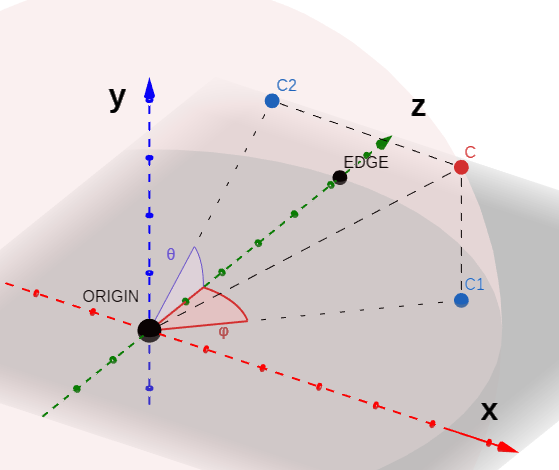
\includegraphics[width=0.9\linewidth]{img/video360/polar_coord.png}
        \caption{Polar coordinates example.}
        \label{fig:polar_coordinates}
    \end{subfigure}
    \begin{subfigure}[b]{0.49\linewidth}
    \centering
        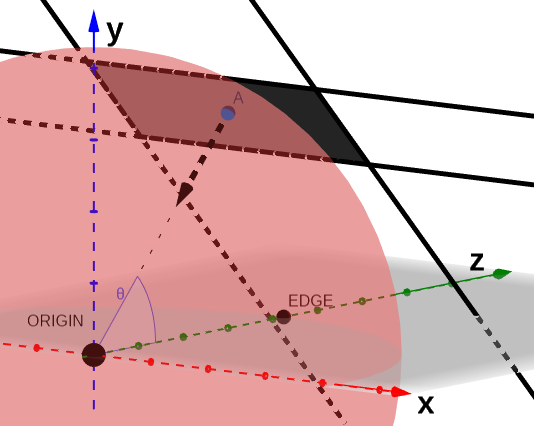
\includegraphics[width=0.9\linewidth]{img/video360/normal_vector.png}
        \caption{Element rotation example.}
        \label{fig:element_rotation}
    \end{subfigure}
    \caption{Polar coordinates system}
\end{figure}

The rotation of a media object is set in a way that the normal vector on the center of its surface points to the origin. By doing so, in any position it is placed, the media object is always facing the viewer. Figure~\ref{fig:element_rotation} shows this rotation, where \emph{A} is the center of the media object.

In the proposed model, each \emph{<scene360>} has always a main 360-degree interactive video. The initial scene in which the application starts is defined by an attribute \emph{entry} in the element <body>. This attribute refers to the \emph{id} attribute of the \emph{<scene360>} element pointing to the main 360-degree video. Media objects inside a 360 scene can be synchronized to the main video~(\textbf{RP.6}). For this, we use SMIL \emph{begin} and \emph{dur} attributes in a media object. These, respectively, define the start time and duration for the presentation of the specified media object.

The \emph{onselect} attribute is used to support user navigation through 360 scenes~(\textbf{RI.1}). This attribute can be defined in any media element, by referencing the \emph{id} of the target scene in its value. Once defined in an element, it transforms it into a navigation element for the referenced scene. Moreover, the \emph{<preview>} defines a viewport of a \emph{<scene360>} using its \emph{id} in the \emph{src}, which can be viewed as a 2D video inside another scene. The temporal segment of the target scene displayed in the preview is defined by the attributes \emph{clipBegin} and \emph{clipEnd}. 

The 360-video might have a particular region of interest to the viewer, which is represented by the \emph{<hotspot>}~(\textbf{RI.2}) element. Meixner \cite{Britta2017} defines a hotspot as an interactive area in a video that invokes an action. The author may create interactions when the user is either looking at it or not. As in the other elements, its position is defined by the \emph{r, phi, theta} attributes. This element has also the attributes \emph{onLookAt} and \emph{duringNotLookingAt}. The attribute \emph{onLookAt} specifies another element to be started once the user looks at the \emph{<hotspot>}. Similarly, the attribute \emph{duringNotLookingAt} specifies another element to be started when the user is not looking at the \emph{<hotspot>} and is stopped once the user looks at it.

The \emph{<mirror>} element refers to picture-in-picture live view of a viewport of the \emph{<scene360>} (\textbf{RI.3}). This viewport is defined using the \emph{src} attribute and assigning it to the \emph{id} of a \emph{<hotspot>} element. Using these elements, authors can define that when the user is staring at a viewport different from the one defined as a \emph{<hotspot>}, the \emph{<mirror>} element will be triggered showing the PiP view at the current user's viewport, attracting his attention to the important section of the 360-degree video. Since the \emph{<mirror>} element refers to a viewport of the current scene, it does not support \emph{onselect} because it would not be intuitive to have an element referring to a scene and navigating to another when selected.


\section{Dynamic Subtitles Positioning in 360-video}
\label{sec:authoring_discussion}

Using the adaptations described in Section \ref{sec:authoring_clustering_360}, we are able to apply \emph{video face clustering} in 360-videos. Figure \ref{fig:360_video_timeline} shows an example of this usage. It contains the two actors present in the 360-video and part of the video's timeline tagged with colors representing the presence of these actors.

\begin{figure}[!ht]
    \centering
    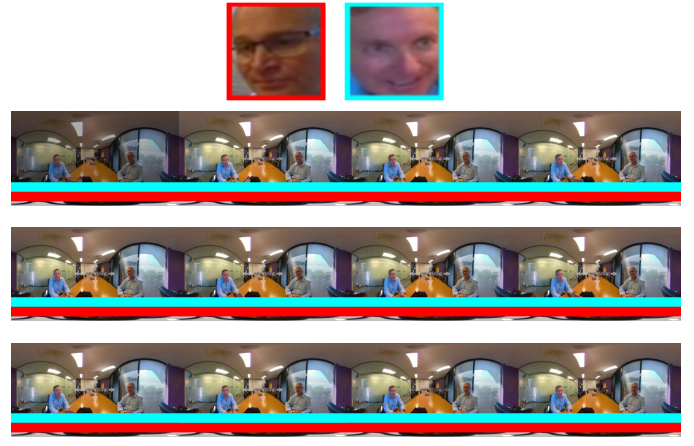
\includegraphics[width=0.8\linewidth]{img/video360/timeline-360.png}
    \caption{360-video timeline tagged by the actors presence. In this case, both actors were present in all frames.}
    \label{fig:360_video_timeline}
\end{figure}

With this clustering, for each actor detected, we generate a file containing the positions in polar coordinates of him/her for each time. By doing so, we use these files for defining the subtitles positioning using our authoring model. Listing \ref{list:ex-subtitles} shows the XML representation of an interactive 360-video with subtitles. In lines 6 and 7, we define subtitles elements, one for each actor. Using the \emph{tpos} attribute, we define that these subtitles follow the actors' positions in the video. As the positions defined in the \emph{tpos} files are relative to the initial position of the subtitle element, we use \emph{theta}=5, so that the subtitles are placed 5 degrees below the center of the actors' faces.


\begin{lstlisting}[
caption={XML representation for 360-video with subtitles following the actors positions.},
frameround=tttt,float=!ht, language=xml, 
label={list:ex-subtitles}, belowskip=-1\baselineskip, basicstyle=\footnotesize ]
<presentation360>
  <head>
  </head>
  <body entry = "boardroom">
    <scene360 id="boardroom" src="boardroom.mp4" volume="1">   
      <subtitle src="actor1.srt" r = "10" theta="5" tpos="actor1-positions.csv"/>      
      <subtitle src="actor2.srt" r = "10" theta="5" tpos="actor2-positions.csv"/>
    </scene360>
  </body>
</presentation360>
\end{lstlisting}

We can also define a more interactive setting for subtitles in 360-video with our authoring model and \emph{Video Face Clustering}. In this new setting, the subtitles follow the actors when they are in the user's viewport, which means that the user can see them. When they are not visible, subtitles are presented at the bottom center of the user's viewport. Listing \ref{list:ex-interactive-subtitles} contains the definition of this setting. 

In the \emph{head}, we define three \emph{styles}. These \emph{styles} contain attributes that can be reused by the elements in the body. The first two \emph{styles}~(lines 3 and 4) define attributes regarding the actor positions in the 360-video with their respective times. These styles are used by the \emph{subtitle} elements on lines 9 and 10 for defining that such subtitles follow the actors' positions. We also define two \emph{hotspot} elements that follow the actor positions~(lines 11 and 12). They are used like triggers with the attribute \emph{duringNotLookingAt} to start the other \emph{subtitles} when the \emph{hotspot} elements~(the actors) are not visible to the user. The other \emph{substile} elements reuse the style defined on line 5. This \emph{style} contains the attribute \emph{followCamera} set to \emph{true}, so that it follows the users head motion. In this way, the \emph{subtitles} defined on lines 13 and 14 follow the user's head motion.


\begin{lstlisting}[
caption={XML representation for 360-video with subtitles following the actors positions.},
frameround=tttt,float=!ht, language=xml, 
label={list:ex-interactive-subtitles}, belowskip=-1\baselineskip, basicstyle=\footnotesize]
<presentation360>
  <head>
    <style id ="sty-actor1" tpos="actor1-positions.csv" begin="0s" r = "10"/>
    <style id ="sty-actor2" tpos="actor2-positions.csv" begin="0s" r = "10"/>
    <style id ="sty-follow" begin ="0s"  theta="20" followCamera="true" r="10"/>
  </head>
  <body entry = "boardroom">
    <scene360 id="boardroom" src="boardroom.mp4" volume="1">      
      <subtitle style="sty-actor1" src="actor1.srt" theta="5"/>      
      <subtitle style="sty-actor2" src="actor2.srt" theta="5"/>
      <hotspot style ="sty-actor1" duringNotLookingAt="sub-follow-actor1"/>
      <hotspot style ="sty-actor2" duringNotLookingAt="sub-follow-actor2"/>
      <subtitle style ="sty-follow" id="sub-follow-actor1" src="actor1.srt"/>
      <subtitle style ="sty-follow" id="sub-follow-actor2" src="actor2.srt"/>
    </scene360>
  </body>
</presentation360>
\end{lstlisting}

Figure \ref{fig:dynamic_subtitles} shows how this setting works. In Figure \ref{subfig:subtitles_actor}, the subtitles are placed close to the actor that is visible in the current user's viewport. When the actor is not visible, as shown in Figure \ref{subfig:subtitles_bottom}, the subtitles are placed at the bottom of the user's viewport. In this way, the user does not lose the content present in the subtitles.

\begin{figure}[!ht]
\centering
    \begin{subfigure}{0.49\linewidth}
        \centering
        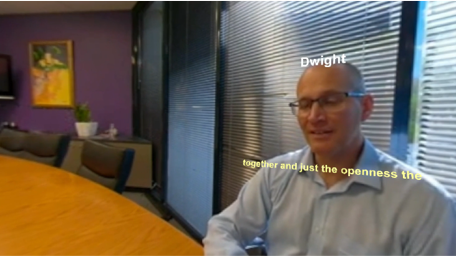
\includegraphics[width=1\textwidth]{img/video360/subtitles_actor.png}
        \caption{Subtitles close to actors' faces when they are in the user's viewport.}
        \label{subfig:subtitles_actor}
    \end{subfigure}\hfill
    \begin{subfigure}{0.49\linewidth}
        \centering
        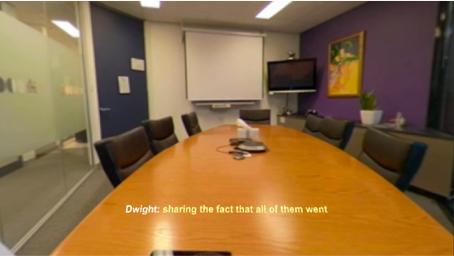
\includegraphics[width=1\textwidth]{img/video360/subtitles_bottom.png}
        \caption{Subtitles positioning in the bottom of user's viewport otherwise.}
        \label{subfig:subtitles_bottom}
    \end{subfigure}

\caption{Dynamic subtitles positioning using video face clustering and our authoring model.}
\label{fig:dynamic_subtitles}
\end{figure}

It is worth noticing that, with this setting, the disadvantage presented in Table \ref{tab:catalog} that the speaker-following subtitles are not always visible to the user is mitigated.

\section{Discussion}

This chapter proposed an automatic way for positioning subtitles in 360-video. This is done with the dynamic placement of subtitles based on the automatic localization of actors. For doing that we use an authoring model for composing and presenting these dynamic subtitles in 360-videos.

Different from traditional 2d-videos, 360-videos are commonly represented using the equirectangular projection. This projection introduces severe distortions that are not easily handled by traditional CNNs. Then, we used an approach based on viewports extraction for the face detection step of \emph{Video Face Clustering}. We first extract viewports from the equirectangular image~(or 360-video frame, in this case) and use MTCNN pre-trained with standard images for face detection in each viewport. Finally, these detections are mapped back to the equirectangular image. We evaluated this approach against MTCNN without viewports in a synthetic equirectangular dataset based on the FDDB benchmark. The usage of viewports achieved better results, especially when considering images with more severe distortions.

In this chapter, we also proposed an authoring model that allows the design and creation of interactive 360-videos. The proposed model is the result of the analysis of different scenarios of immersive 360 multimedia applications. Besides supporting dynamic subtitles positioning in 360-videos, it also supports navigation among 360-videos, additional media, interactive behaviors such as selection and guided attention. For other case studies not closely related to this dissertation, please check our paper that presents this authoring model~\cite{mendes2020authoring}. This model is supported by a player based on the Unity Game Engine.\footnote{\url{https://github.com/TeleMidia/VR360Authoring}}

